\documentclass[10pt]{beamer}
\usetheme[
%%% options passed to the outer theme
%    hidetitle,           % hide the (short) title in the sidebar
%    hideauthor,          % hide the (short) author in the sidebar
%    hideinstitute,       % hide the (short) institute in the bottom of the sidebar
%    shownavsym,          % show the navigation symbols
%    width=2cm,           % width of the sidebar (default is 2 cm)
%    hideothersubsections,% hide all subsections but the subsections in the current section
%    hideallsubsections,  % hide all subsections
    left               % right of left position of sidebar (default is right)
%%% options passed to the color theme
%    lightheaderbg,       % use a light header background
  ]{AAUsidebar}

% If you want to change the colors of the various elements in the theme, edit and uncomment the following lines
% Change the bar and sidebar colors:
%\setbeamercolor{AAUsidebar}{fg=red!20,bg=red}
%\setbeamercolor{sidebar}{bg=red!20}
% Change the color of the structural elements:
%\setbeamercolor{structure}{fg=red}
% Change the frame title text color:
%\setbeamercolor{frametitle}{fg=blue}
% Change the normal text color background:
%\setbeamercolor{normal text}{bg=gray!10}
% ... and you can of course change a lot more - see the beamer user manual.


\usepackage[utf8]{inputenc}
\usepackage[english]{babel}
\usepackage[T1]{fontenc}
\usepackage{multimedia}
% Or whatever. Note that the encoding and the font should match. If T1
% does not look nice, try deleting the line with the fontenc.
\usepackage{helvet}
\usepackage{tikz}
\usetikzlibrary{shapes,shapes.geometric, arrows,positioning,calc}
\tikzset{
	block/.style = {draw, fill=white, rectangle, minimum height=3em, minimum width=3em},
	tmp/.style  = {coordinate}, 
	sum/.style= {draw, fill=white, circle, node distance=1cm},
	input/.style = {coordinate},
	output/.style= {coordinate},
	pinstyle/.style = {pin edge={to-,thin,black}
	}
}

\usepackage{amsmath}
\usepackage{amssymb}

% colored hyperlinks
\newcommand{\chref}[2]{%
  \href{#1}{{\usebeamercolor[bg]{AAUsidebar}#2}}%
}

\title[Modelling and Networked Control of Water Distribution Networks]% optional, use only with long paper titles
{This is the title i think}

% \subtitle{}  % could also be a conference name

\date{\today}

\author[CA834] % optional, use only with lots of authors
{
  CA834
}
% - Give the names in the same order as they appear in the paper.
% - Use the \inst{?} command only if the authors have different
%   affiliation. See the beamer manual for an example

\institute[
%  {\includegraphics[scale=0.2]{aau_segl}}\\ %insert a company, department or university logo
  Control and Automation\\
  Aalborg University\\
  Denmark
] % optional - is placed in the bottom of the sidebar on every slide
{% is placed on the title page
  Control and Automation, Group 834\\
  Aalborg University\\
  Denmark
  
  %there must be an empty line above this line - otherwise some unwanted space is added between the university and the country (I do not know why;( )
}


% specify a logo on the titlepage (you can specify additional logos an include them in 
% institute command below
\pgfdeclareimage[height=1.5cm]{titlepagelogo}{AAUgraphics/aau_logo_new} % placed on the title page
%\pgfdeclareimage[height=1.5cm]{titlepagelogo2}{graphics/aau_logo_new} % placed on the title page
\titlegraphic{% is placed on the bottom of the title page
  \pgfuseimage{titlepagelogo}
%  \hspace{1cm}\pgfuseimage{titlepagelogo2}
}


\begin{document}
% the titlepage
{\aauwavesbg%
\begin{frame}[plain,noframenumbering] % the plain option removes the sidebar and header from the title page
  \titlepage
\end{frame}}
%%%%%%%%%%%%%%%%

% TOC
\begin{frame}{Agenda}{}
\tableofcontents
\end{frame}
%%%%%%%%%%%%%%%%

\section{Introduction}


% motivation for creating this theme
\begin{frame}{Introduction}{Introduction to Reefer Trailer}
\begin{itemize}
	\item First item of an itemize 
	\item Second item with subitems:
	\begin{itemize}
		\item Subitem 1 i think
		\item Subitem 2 i think
	\end{itemize}

\end{itemize}
\end{frame}

\begin{frame}{Introduction}{A reefer trailer}
\begin{block}{}
	A reefer trailer is modelled and controlled:
	
	\begin{figure}[h]
		\centering
		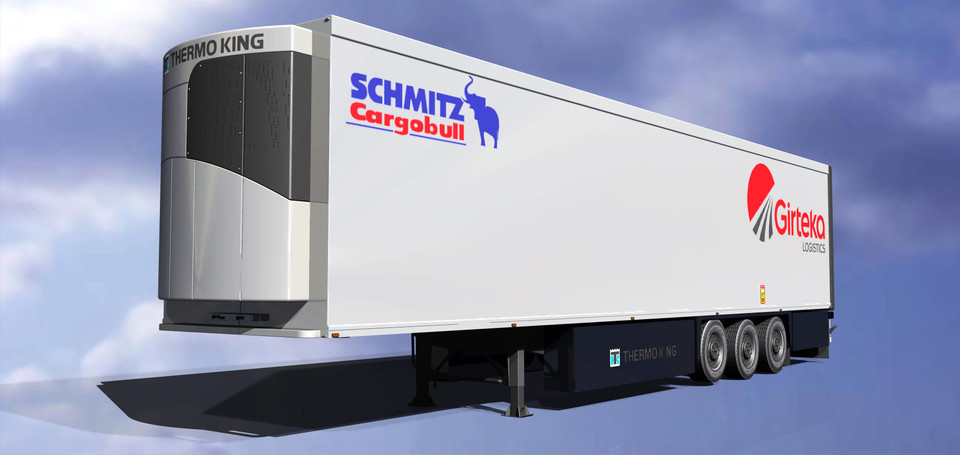
\includegraphics[width=0.5\linewidth]{../Graphics/3d_draw_trailer.jpg}
		\label{fig:trailer}
		
	\end{figure}
\end{block}

\begin{block}{}
	A reefer trailer.
\end{block}


\end{frame}
%%%%%%%%%%%%%%%%

% ======================================================================
% Inputs for topics here!

\section{Modelling of WDN}


\subsection{Fast Dynamics and Graph theory}
%\input{Topics/SystemModel/Model}
%
\subsection{Slow Dynamics and Linearisation}
%\input{Topics/SlowDynamicsLinearisation/SlowDynamicsLinearisation}
%
\section{Template test}
\begin{frame}{Title}{Subtitle}
	 \textbf{Some text}
	 \begin{itemize}
	 	\item Item
	 \end{itemize}
\end{frame}

%%%%%%%%%%%%%%%%%

\begin{frame}{Next slide title}{Next slide subtitle}
	 \textbf{Some text}
	\begin{itemize}
		\item Item
	\end{itemize}
\end{frame}

%%%%%%%%%%%%%%%%%















% ======================================================================




\section{References}
\begin{frame}{References}
	\bibliographystyle{ieeetran}
	\bibliography{../../RefLib/CA7Projekt.bib}
\end{frame}

{\aauwavesbg
\begin{frame}[plain,noframenumbering]
  \finalpage{Open for questions!}
\end{frame}}
%%%%%%%%%%%%%%%%

\end{document}
